

\subsection{Tick Options}

\subsubsection{Tick Coordinates and Label Texts}
\begin{pgfplotsxykey}{\x tick=\mchoice{\textbackslash empty,data,\normalfont\marg{coordinate list}} (initially \marg{})}
These options assign a list of \emph{positions} where ticks shall be placed. The argument is either the empty string (which is the initial value), the command |\empty|, the special string `|data|' or a list of coordinates. The initial configuration of an empty string means to generate these positions automatically. The choice |\empty| will result in no tick at all. The special value `|data|' will produce tick marks at every coordinate of the first plot. Otherwise, tick marks will be placed at every coordinate in  \meta{coordinate list}.

The \meta{coordinate list} will be used inside of a |\foreach \x in |\marg{coordinate list} statement. The format is as follows:
\begin{itemize}
	\item |{0,1,2,5,8,1e1,1.5e1}| (a series of coordinates),
	\item |{0,...,5}| (the same as |{0,1,2,3,4,5}|),
	\item |{0,2,...,10}| (the same as |{0,2,4,6,8,10}|),
	\item |{9,...,3.5}| (the same as |{9, 8, 7, 6, 5, 4}|),
	\item See \cite[Section~34]{tikz} for a more detailed definition of the options.
	\item Please be careful with white spaces inside of \meta{coordinate list} (at least around the dots).
\end{itemize}
For logplots, \PGFPlots\ will apply $\log(\cdot)$ to each element in `\meta{coordinate list}' (similarly, any custom transformations are applied to the argument list). 
\begin{codeexample}[]
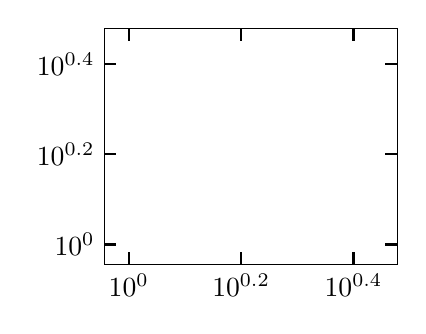
\begin{tikzpicture}
	\begin{loglogaxis}[xtick={12,9897,1468864}]
	% see above for this macro:
	\plotcoords
	\end{loglogaxis}
\end{tikzpicture}
\end{codeexample}

\begin{codeexample}[]
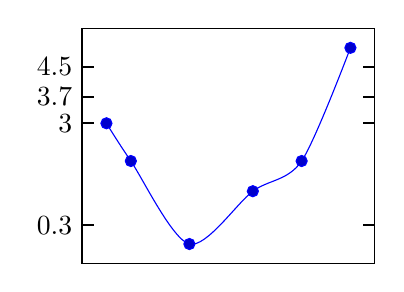
\begin{tikzpicture}
\begin{axis}[
	xtick=\empty,
	ytick={-2,0.3,3,3.7,4.5}]
\addplot+[smooth] coordinates {
	(-2,3) (-1.5,2) (-0.3,-0.2) 
	(1,1.2) (2,2) (3,5)};
\end{axis}
\end{tikzpicture}
\end{codeexample}

\paragraph{Attention:} You can't use the `|...|' syntax if the elements are too large for \TeX! For example, `|xtick=1.5e5,2e7,3e8|' will work (because the elements are interpreted as strings, not as numbers), but `|xtick=1.5,3e5,...,1e10|' will fail because it involves real number arithmetics beyond \TeX's capacities.
\vspace*{0.3cm}

\noindent
The default choice for tick \emph{positions} in normal plots is to place a tick at each coordinate~$i\cdot h$. The step size~$h$ depends on the axis scaling and the axis limits. It is chosen from a list of ``feasible'' step sizes such that neither too much nor too few ticks will be generated. The default for logplots is to place ticks at positions $10^i$ in the axis' range. The positions depend on the axis scaling and the dimensions of the picture. If log plots contain just one (or two) positions $10^i$ in their limits, ticks will be placed at positions $10^{i\cdot h}$ with ``feasible'' step sizes $h$ as in the case of linear axis.

\noindent
The tick \emph{appearance} can be (re)configured with
\begin{codeexample}[code only]
\pgfplotsset{tick style={very thin,gray}}% modifies the style `every tick'
\pgfplotsset{minor tick style={black}}   % modifies the style `every minor tick'
\end{codeexample}

These style commands can be used at any time. The tick line width can be configured with `|major tick length|' and `|minor tick length|'.

\begin{codeexample}[]
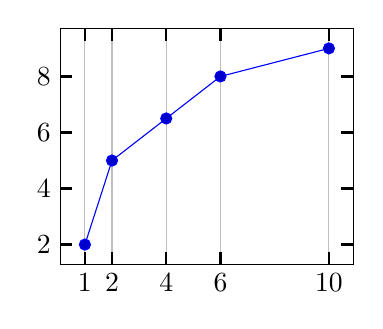
\begin{tikzpicture}
\begin{axis}[xtick=data,xmajorgrids]
	\addplot coordinates {
		(1,2)
		(2,5)
		(4,6.5)
		(6,8)
		(10,9)
	};
\end{axis}
\end{tikzpicture}
\end{codeexample}

\begin{codeexample}[]
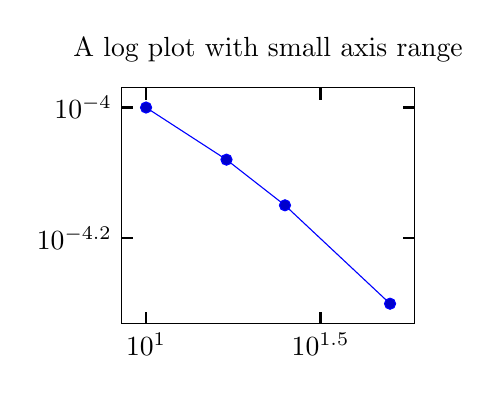
\begin{tikzpicture}
\begin{loglogaxis}[
	title=A log plot with small axis range]

	\addplot coordinates {
		(10,1e-4)
		(17,8.3176e-05)
		(25,7.0794e-05)
		(50,5e-5)
	};
\end{loglogaxis}
\end{tikzpicture}
\end{codeexample}
\end{pgfplotsxykey}

\begin{pgfplotsxykeylist}{minor \x\ tick num=\marg{number} (initially 0),minor tick num=\marg{number}}
	Sets the number of minor tick lines used either for single axes or for all of them.

	Minor ticks will be disabled if the major ticks don't have the same distance and they are currently only available for linear axes (not for logarithmic ones).

\begin{codeexample}[]
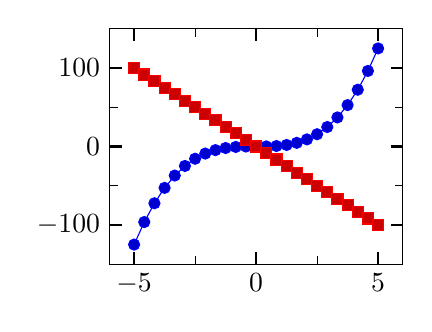
\begin{tikzpicture}
	\begin{axis}[minor tick num=1]
	\addplot {x^3};
	\addplot {-20*x};
	\end{axis}
\end{tikzpicture}
\end{codeexample}

\begin{codeexample}[]
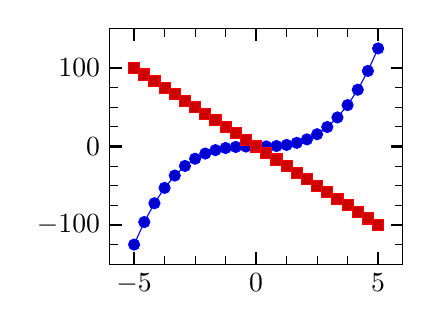
\begin{tikzpicture}
	\begin{axis}[minor tick num=3]
	\addplot {x^3};
	\addplot {-20*x};
	\end{axis}
\end{tikzpicture}
\end{codeexample}

\begin{codeexample}[]
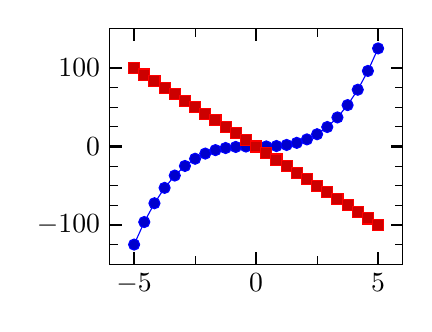
\begin{tikzpicture}
	\begin{axis}[minor x tick num=1,
	             minor y tick num=3]
	\addplot {x^3};
	\addplot {-20*x};
	\end{axis}
\end{tikzpicture}
\end{codeexample}

\end{pgfplotsxykeylist}

\begin{pgfplotsxykeylist}{minor \x tick=\mchoice{data,\normalfont\marg{coordinate list}} (initially empty),%
	minor tick=\mchoice{data,\normalfont\marg{coordinate list}}}
	Allows to provide a list of minor tick positions manually. The syntax is almost the same as for |xtick| or |ytick|: simply provide either a comma--separated list of tick positions or the special value |data|. An empty argument argument disables the |minor tick| feature (in contrast to |xtick| where the special value |\empty| clears the list and an empty argument causes \PGFPlots\ to compute a default tick list).

	In contrast to |minor x tick num|, this key allows to provide \emph{non--uniform} minor tick positions.

\begin{codeexample}[]
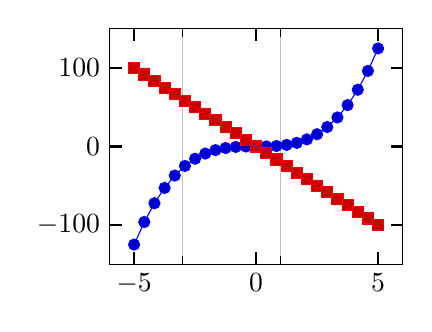
\begin{tikzpicture}
	\begin{axis}[minor xtick={-3,1},grid=minor]
	\addplot {x^3};
	\addplot {-20*x};
	\end{axis}
\end{tikzpicture}
\end{codeexample}

\begin{codeexample}[]
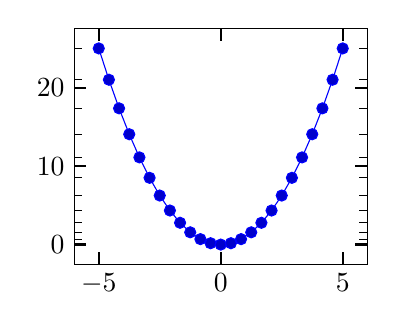
\begin{tikzpicture}
	\begin{axis}[minor ytick=data]
	\addplot {x^2};
	\end{axis}
\end{tikzpicture}
\end{codeexample}

	This key has precedence over |minor x tick num| and its variants; if both of them are given, |minor xtick| is preferred and |minor x tick num| is ignored.
\end{pgfplotsxykeylist}

\begin{pgfplotsxykey}{extra \x\ ticks=\marg{coordinate list}}
Adds \emph{additional} tick positions and tick labels to the $x$~or~$y$ axis. `Additional' tick positions do not affect the normal tick placement algorithms, they are drawn after the normal ticks. This has two benefits: first, you can add single, important tick positions without disabling the default tick label generation and second, you can draw tick labels `on top' of others, possibly using different style flags.


\begin{codeexample}[]
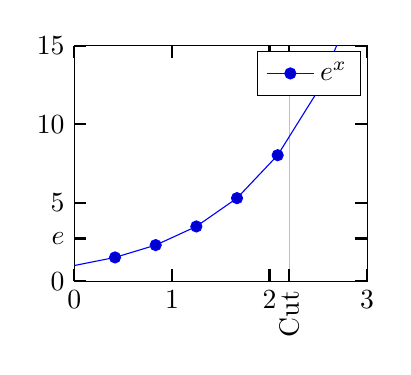
\begin{tikzpicture}
\begin{axis}[
	xmin=0,xmax=3,ymin=0,ymax=15,
	extra y ticks={2.71828},
	extra y tick labels={$e$},
	extra x ticks={2.2},
	extra x tick style={grid=major,
		tick label style={
			rotate=90,anchor=east}},
	extra x tick labels={Cut},
]
	\addplot {exp(x)};
	\addlegendentry{$e^x$}
\end{axis}
\end{tikzpicture}
\end{codeexample}

\message{Overfull hbox is ok.}%
\begin{codeexample}[]
\pgfplotsset{every axis/.append style={width=5.3cm}}
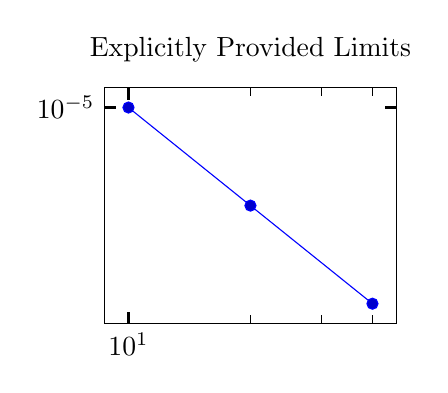
\begin{tikzpicture}
\begin{loglogaxis}[
	title=Explicitly Provided Limits,
	xtickten={1,2},
	ytickten={-5,-6}]
\addplot coordinates 
	{(10,1e-5) (20,5e-6) (40,2.5e-6)};
\end{loglogaxis}
\end{tikzpicture}

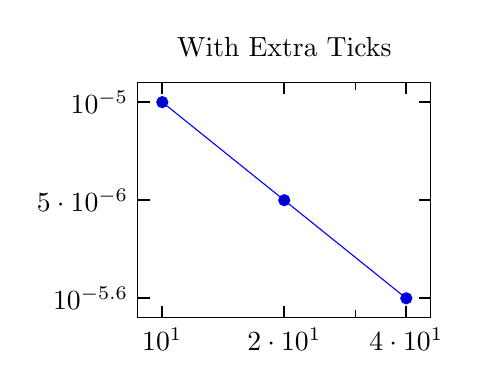
\begin{tikzpicture}
\begin{loglogaxis}[
	title=With Extra Ticks,
	xtickten={1,2},
	ytickten={-5,-6},
	extra x ticks={20,40},
	extra y ticks={5e-6,2.5e-6}]
\addplot coordinates 
	{(10,1e-5) (20,5e-6) (40,2.5e-6)};
\end{loglogaxis}
\end{tikzpicture}

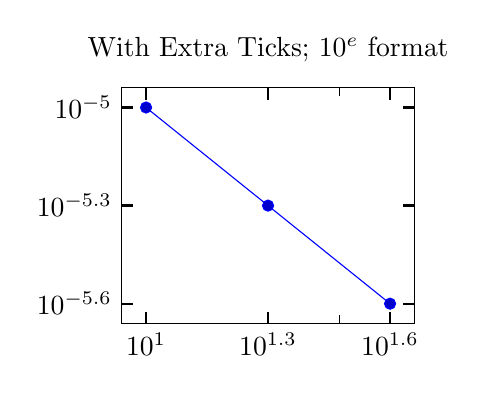
\begin{tikzpicture}
\begin{loglogaxis}[
	title=With Extra Ticks; $10^e$ format,
	extra tick style={log identify minor tick positions=false},
	xtickten={1,2},
	ytickten={-5,-6},
	extra x ticks={20,40},
	extra y ticks={5e-6,2.5e-6}]
\addplot coordinates 
	{(10,1e-5) (20,5e-6) (40,2.5e-6)};
\end{loglogaxis}
\end{tikzpicture}
\end{codeexample}

Remarks:
\begin{itemize} 
\item Use |extra x ticks| to highlight special tick positions. The use of |extra x ticks| does not affect minor tick/grid line generation, so you can place extra ticks at positions $j\cdot 10^i$ in log--plots. 
\item Extra ticks are always typeset as major ticks.

They are affected by |major tick length| or options like |grid=major|.
\item Use the style |every extra x tick| (|every extra y tick|) to configure the appearance.
\item You can also use `|extra x tick style=|\marg{...}' which has the same effect.
\end{itemize}
\end{pgfplotsxykey}

\begin{pgfplotsxykey}{\x tickten=\marg{exponent base 10 list}}
These options allow to place ticks at selected positions $10^k, k \in \text{\marg{exponent base 10 list}}$. They are only used for logplots. The syntax for \marg{exponent base 10 list} is the same as above for |xtick=|\marg{list} or |ytick=|\marg{list}.

Using `|xtickten={1,2,3,4}|' is equivalent to `|xtick={1e1,1e2,1e3,1e4}|', but it requires fewer computational time and it allows to use the short syntax `|xtickten={1,...,4}|'.
\begin{codeexample}[]
\begin{tikzpicture}
\begin{semilogyaxis}[
	samples=8,
	ytickten={-6,-4,...,4},
	domain=0:10]

\addplot {2^(-2*x + 6)};
\addlegendentry{$2^{-2x + 6}$}

% or invoke gnuplot to generate coordinates:
\addplot gnuplot[id=pow2] 
	{2**(-1.5*x -3)};
\addlegendentry{$2^{-1.5x -3}$}
\end{semilogyaxis}
\end{tikzpicture}
\end{codeexample}

In case |log basis x|$\neq 10$, the meaning of |xtickten| changes. In such a case, |xtickten| will still assign the exponent, but for the chosen |log basis x| instead of base $10$.
\end{pgfplotsxykey}

\begin{pgfplotsxykey}{\x ticklabels=\marg{label list}}
\label{pgfplots:key:xticklabels}%
Assigns a \emph{list} of tick \emph{labels} to each tick position. Tick \emph{positions} are assigned using the |xtick| and |ytick|-options.

This is one of two options to assign tick labels directly. The other option is |xticklabel=|\marg{command} (or |yticklabel=|\marg{command}).
The option `|xticklabel|' offers higher flexibility while `|xticklabels|' is easier to use. See also the variant |xticklabels from table|.

The argument \meta{label list} has the same format as for ticks, that means
\begin{codeexample}[code only]
xticklabels={$\frac{1}{2}$,$e$}
\end{codeexample}
denotes the two--element--list $\{\frac 12, e\}$. The list indices match the indices of the tick positions. If you need commas inside of list elements, use 
\begin{codeexample}[code only]
xticklabels={{0,5}, $e$}.
\end{codeexample}


\begin{codeexample}[]
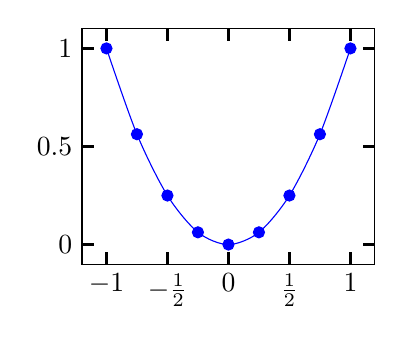
\begin{tikzpicture}
\begin{axis}[
	xtick={-1.5,-1,...,1.5},
	xticklabels={%
		$-1\frac 12$,
		$-1$,
		$-\frac 12$,
		$0$,
		$\frac 12$,
		$1$},
	% note: \frac can be done automatically:
	% xticklabel style={/pgf/number format/frac},
]
\addplot[smooth,blue,mark=*] 
coordinates {
	(-1,    1)
	(-0.75, 0.5625)
	(-0.5,  0.25)
	(-0.25, 0.0625)
	(0,     0)
	(0.25,  0.0625)
	(0.5,   0.25)
	(0.75,  0.5625)
	(1,     1)
};
\end{axis}
\end{tikzpicture}
\end{codeexample}

\begin{codeexample}[]
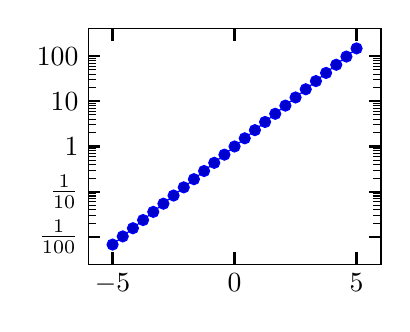
\begin{tikzpicture}
\begin{semilogyaxis}[
  ytickten={-2,-1,0,1,2},
  yticklabels={$\frac{1}{100}$,%
  	$\frac{1}{10}$,%
	1,10,100},
]
	\addplot {exp(x)};
\end{semilogyaxis}
\end{tikzpicture}
\end{codeexample}

	Note that it is also possible to terminate list entries with two backslashes, |\\|. In that case, the last entry needs to be terminated by |\\| as well (it is the same alternative syntax which is also accepted for |\legend| and |cycle list|).

	Please keep in mind that the arguments \emph{always} refer the a list of tick positions, although it does not alter or define the list of positions. Consequently, you should also provide the list of positions. Note that a list of positions might be longer than what is actually displayed (in case the axis limits clip some of the value away), but the index mapping into \meta{label list} still includes the clipped values.
\end{pgfplotsxykey}


\begin{pgfplotsxykey}{\x ticklabel=\marg{command}}
These keys change the \TeX-command which creates the tick \emph{labels} assigned to each tick position (see options |xtick| and |ytick|). 

This is one of the two options to assign tick labels directly. The other option is `|xticklabels=|\marg{label list}' (or |yticklabels=|\marg{label list}). The option `|xticklabel|' offers higher flexibility while `|xticklabels|' is easier to use.

The argument \meta{command} can be any \TeX-text. The following commands are valid inside of \meta{command}:
\begin{description}
	\item[] \declareandlabel{\tick} The current element of option |xtick| (or |ytick|).
	\item[] \declareandlabel{\ticknum} The current tick number, starting with~0 (it is a macro containing a number).
	\item[] \declareandlabel{\nexttick} This command is only valid if the |x tick label as interval| option is set (or the corresponding variable for~$y$). It will contain the position of the next tick position, that means the right boundary of the tick interval.
\end{description}
The default argument is 
\begin{itemize}
	\item \declareandlabel{\axisdefaultticklabel} for normal plots:
\begin{codeexample}[code only]
\def\axisdefaultticklabel{$\pgfmathprintnumber{\tick}$}
\end{codeexample}

	\item \declareandlabel{\axisdefaultticklabellog} for logplots:
\begin{codeexample}[code only]
\def\axisdefaultticklabellog{%
	\pgfkeysgetvalue{/pgfplots/log number format code/.@cmd}\pgfplots@log@label@style
	\expandafter\pgfplots@log@label@style\tick\pgfeov
}
\end{codeexample}
\end{itemize}
That means you can configure the appearance of linear axis with the number formatting options described in Section~\ref{sec:number:printing} and logarithmic axis with |log number format code|, see below.

\begin{codeexample}[]
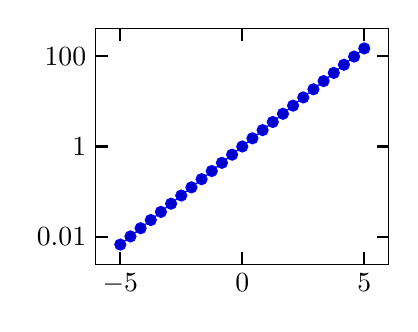
\begin{tikzpicture}
	\begin{semilogyaxis}[
		yticklabel style={/pgf/number format/fixed},
		% changes tick labels to a number instead 
		% of exponential notation:
		yticklabel={%
			\pgfmathfloatparsenumber{\tick}%
			\pgfmathfloatexp{\pgfmathresult}%
			\pgfmathprintnumber{\pgfmathresult}%
		},
	]
		\addplot {exp(x)};
	\end{semilogyaxis}
\end{tikzpicture}
\end{codeexample}

The following example uses explicitly formatted $x$ tick labels and a small \TeX\ script to format $y$ tick labels as fractions in the form \meta{sign}\meta{number}|/10| (note that the |/pgf/number format/frac| style can do similar things automatically, see \PGFPlotstable\ and the documentation therein).
% \usepackage{nicefrac}
\begin{codeexample}[width=4cm]
% \usepackage{nicefrace}% required
\begin{tikzpicture}
\begin{axis}[
	% x ticks explicitly formatted:
	xtick={0,1,0.5,0.25,0.75},
	xticklabels={$0$,$1$,$\frac12$,$\frac14$,$\frac34$},
	% y ticks automatically by some code fragment:
	ytick=data,
	yticklabel={%
		\scriptsize
		\ifdim\tick pt<0pt % a TeX \if -- see TeX Book
			\pgfmathparse{-10*\tick}%
			$-\nicefrac{\pgfmathprintnumber{\pgfmathresult}}{10}$%
		\else
			\ifdim\tick pt=0pt
			\else
				\pgfmathparse{10*\tick}%
				$\nicefrac{\pgfmathprintnumber{\pgfmathresult}}{10}$%
			\fi
		\fi
	},
	% NOTE: this here does the same:
	% yticklabel style={/pgf/number format/.cd,frac,
	% 	frac TeX=\nicefrac,frac whole=false,frac denom=10},
	ymajorgrids,
	title=A special Prewavelet,
	axis x line=center,
	axis y line=left,
	]
	\addplot coordinates {(0,-1.2) (0.25,1.1) 
		(0.5,-0.6) (0.75,0.1) (1,0)};
\end{axis}
\end{tikzpicture}
\end{codeexample}
\noindent The \TeX\ script takes the |\tick| macro as input and applies some logic. The |\ifdim\tick pt<0pt| means ``if dimension |\tick pt| $ < $ |0pt|''. The |\ifdim| is \TeX's only way to compare real fixed point numbers and the author did not want to invoke |\pgfmath| for this simple task. Since |\ifdim| expects a dimension, we have to use the |pt| suffix which is compatible with |\pgfmath|. The result is that negative numbers, zero and positive numbers are typeset differently.

You can change the appearance of tick labels with
\begin{codeexample}[code only]
\pgfplotsset{tick label style={
	font=\tiny,
	/pgf/number format/sci}}% this modifies the `every tick label' style
\end{codeexample}
and/or
\begin{codeexample}[code only]
\pgfplotsset{x tick label style={
	above,
	/pgf/number format/fixed zerofill}}% this modifies the `every x tick label' style
\end{codeexample}
and
\begin{codeexample}[code only]
\pgfplotsset{y tick label style={font=\bfseries}}% modifies `every y tick label'
\end{codeexample}
\end{pgfplotsxykey}

\begin{pgfplotsxykey}{\x ticklabels from table=\marg{\textbackslash table or filename}\marg{colname}}
	A variant of |xticklabels=|\marg{list} which uses each entry in the column named \meta{colname} from a table as tick labels.

	The first argument \meta{\textbackslash table or filename} can be either a loaded table macro (i.e.\ the result of |\pgfplotstableread|\marg{file name}\marg{\textbackslash table}) or just a file name.

	The second argument can be a column name, a column alias or a |create on use| specification (see \PGFPlotstable\ for the latter two). Furthermore, it can be |[index]|\meta{integer} in which case \meta{integer} is a column index.

	The behavior of |xticklabels from table| is the same as if the column \meta{colname} would have been provided as comma separated list to |xticklabels|. This means the column can contain text, \TeX\ macros or even math mode.

	If you have white spaces in your cells, enclose the complete cell in curly braces, |{example cell}|. The detailed input format for tables is discussed in \verbpdfref{\addplot table} and in the documentation for \PGFPlotstable.
\end{pgfplotsxykey}

\begin{pgfplotsxykey}{extra \x\ tick label=\marg{\TeX\ code}}
	As |xticklabel| provides code to generate tick labels for each |xtick|, the key |extra x tick label| provides code to generate tick labels for every element in |extra x ticks|.
\end{pgfplotsxykey}

\begin{pgfplotsxykey}{extra \x\ tick labels=\marg{label list}}
	As |xticklabels| provides explicit tick labels for each |xtick|, the key |extra x tick labels| provides explicit tick labels for every element in |extra x ticks|.
\end{pgfplotsxykey}



\begin{pgfplotsxykey}{\x\ tick label as interval=\mchoice{true,false} (initially false)}
\label{key:pgfplots:ticklabelasinterval}
	Allows to treat tick labels as intervals; that means the tick positions denote the interval boundaries. If there are $n$ positions, $(n-1)$ tick labels will be generated, one for each interval.
\begin{codeexample}[]
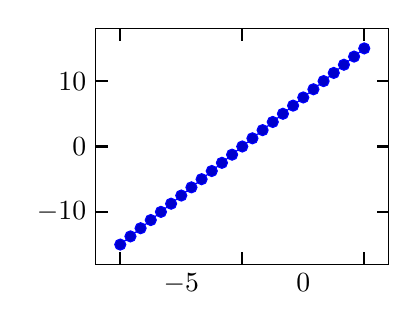
\begin{tikzpicture}
\begin{axis}[x tick label as interval]
	\addplot {3*x};
\end{axis}
\end{tikzpicture}
\end{codeexample}
	This mode enables the use of |\nexttick| inside of |xticklabel| (or |yticklabel|). A common application might be a bar plot.
\begin{codeexample}[]
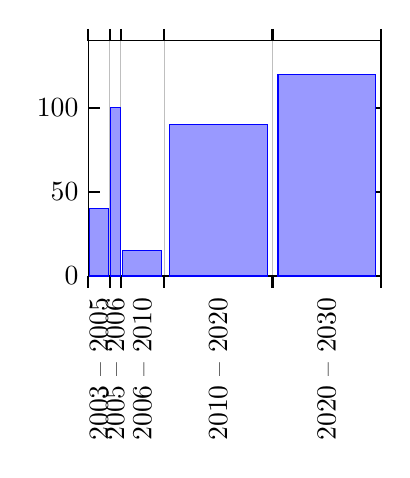
\begin{tikzpicture}
\begin{axis}[
	ybar interval=0.9,
	x tick label as interval,
	xmin=2003,xmax=2030,
	ymin=0,ymax=140,
	xticklabel={
	   $\pgfmathprintnumber{\tick}$
	-- $\pgfmathprintnumber{\nexttick}$},
	xtick=data,
	x tick label style={
		rotate=90,anchor=east,
		/pgf/number format/1000 sep=}
]

	\addplot[draw=blue,fill=blue!40!white]
		coordinates
		{(2003,40) (2005,100) (2006,15) 
		 (2010,90) (2020,120) (2030,3)};
\end{axis}
\end{tikzpicture}
\end{codeexample}
\end{pgfplotsxykey}



\begin{pgfplotsxykeylist}{\x minorticks=\mchoice{true,false} (initially true),\x majorticks=\mchoice{true,false} (initially true),ticks=\mchoice{minor,major,both,none} (initially both)}
Enables/disables the small tick lines either for single axis or for all of them. Major ticks are those placed at the tick positions and minor ticks are between tick positions. Please note that minor ticks are automatically disabled if |xtick| is not a uniform range\footnote{A uniform list means the difference between all elements is the same for linear axis or, for logarithmic axes, $\log(10)$.}.

The key |minor tick length=|\marg{dimen} configures the tick length for minor ticks while the |major| variant applies to major ticks.
You can configure the appearance using the following styles:
\begin{codeexample}[code only]
\pgfplotsset{every tick/.append style={color=black}} % applies to major and minor ticks,
\pgfplotsset{every minor tick/.append style={thin}}  % applies only to minor ticks,
\pgfplotsset{every major tick/.append style={thick}} % applies only to major ticks.
\end{codeexample}
There is also the style ``|every tick|'' which applies to both, major and minor ticks.
\end{pgfplotsxykeylist}

\begin{pgfplotsxykeylist}{\x tickmin=\marg{coord}, \x tickmax=\marg{coord}}
	These keys can be used to modify minimum/maximum values before ticks are drawn. Because this applies to axis discontinuities, it is described on page~\pageref{key:xytickminmax} in Section~\ref{key:xytickminmax}, ``Axis Discontinuities"'.
\end{pgfplotsxykeylist}

\subsubsection{Tick Alignment: Positions and Shifts}

\begin{pgfplotsxykeylist}{\x tick pos=\mchoice{left,right,both} (initially both),tick pos=\mchoice{left,right,both}}
Allows to choose where to place the small tick lines. In the default configuration, this does also affect tick \emph{labels}, see below. The |tick pos| style sets all of them to the same value (aliased by |tickpos|\pgfmanualpdflabel{/pgfplots/tickpos}). This option is only useful for boxed axes.

For $x$, the additional choices |bottom| and |top| can be used which are equivalent to |left| and |right|, respectively. Both are accepted for $y$.

Changing |tick pos| will also affect the placement of tick labels. 

Note that it can also affect the |axis lines| key, although not all combinations make sense. Make sure the settings are consistent.
\end{pgfplotsxykeylist}

\begin{pgfplotsxykeylist}{%
	\x ticklabel pos=\mchoice{left,right,default} (initially default),
	   ticklabel pos=\mchoice{left,right,default} (initially default)}
Allows to choose where to place tick \emph{labels}. The choices |left| and |right| place tick labels either at the left or at the right side of the complete axis. The choice |default| uses the same setting as |xtick pos| (or |ytick pos|). This option is only useful for boxed axes -- keep it to |default| for non-boxed figures. The |ticklabel pos| style sets all three of them to the same value.

For $x$, the additional choices |bottom| and |top| can be used which are equivalent to |left| and |right|, respectively. Both are accepted for $x$.
\end{pgfplotsxykeylist}

\begin{pgfplotsxykeylist}{%
	\x tick align=\mchoice{inside,center,outside} (initially inside),
	   tick align=\mchoice{inside,center,outside} (initially inside)}
Allows to change the location of the ticks relative to the axis lines. The |tick align| sets all of them to the same value.
Default is ``|inside|''.
\begin{codeexample}[]
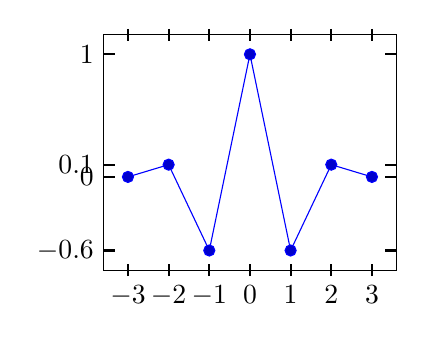
\begin{tikzpicture}
\begin{axis}[
	xtick=data,ytick=data,
	xtick align=center]
\addplot coordinates 
	{(-3,0) (-2,0.1) (-1,-0.6) 
	 (0,1)
	 (1,-0.6) (2,0.1) (3,0)};
\end{axis}
\end{tikzpicture}
\end{codeexample}

\begin{codeexample}[]
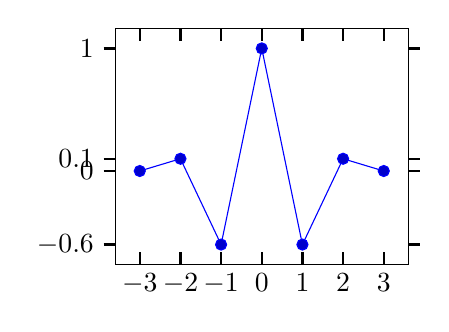
\begin{tikzpicture}
\begin{axis}[
	xtick=data,ytick=data,
	ytick align=outside]
\addplot coordinates 
	{(-3,0) (-2,0.1) (-1,-0.6)
	 (0,1) 
	 (1,-0.6) (2,0.1) (3,0)};
\end{axis}
\end{tikzpicture}
\end{codeexample}

These tick alignment options are set automatically by the |axis x line| and |axis y line| methods (unless one appends an asterisk `|*|'):
\begin{codeexample}[]
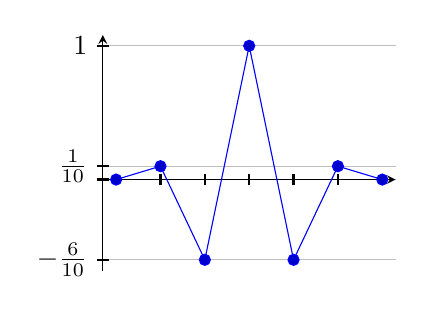
\begin{tikzpicture}
\begin{axis}[
	xtick=data,
	axis x line=center,
	xticklabels={,,},
	ytick={-0.6,0,0.1,1},
	yticklabels={
		$-\frac{6}{10}$,,
		$\frac{1}{10}$,$1$},
	ymajorgrids,
	axis y line=left,
	enlargelimits=0.05]
\addplot coordinates 
	{(-3,0) (-2,0.1) (-1,-0.6)
	 (0,1) 
	 (1,-0.6) (2,0.1) (3,0)};
\end{axis}
\end{tikzpicture}
\end{codeexample}

\end{pgfplotsxykeylist}

\begin{pgfplotsxykeylist}{%
	\x ticklabel shift=\marg{dimension} (initially empty),%
	   ticklabel shift=\marg{dimension} (initially empty)}
	Shifts tick labels in direction of the outer unit normal of the axis by an amount of \meta{dimension}. The |ticklabel shift| sets the same value for all axes.

	This is usually unnecessary as the |anchor| of a tick label already yields enough spacing in most cases.
\end{pgfplotsxykeylist}

\subsubsection{Tick Scaling - Common Factors In Ticks}
\label{sec:scaled:ticks}%
\begin{pgfplotsxykeylist}{
	scaled ticks=\mchoice{true,false,base 10:{\normalfont\meta{e}},real:{\normalfont\meta{num}},manual:{\normalfont\marg{label}\marg{code}}} (initially true),%
	scaled \x\ ticks=\meta{one of the values} (initially true)%
}
Allows to factor out common exponents in tick labels for \emph{linear axes}. For example, if you have tick labels $20000,40000$ and $60000$, you may want to save some space and write $2,4,6$ with a separate factor `$\cdot 10^4$'. Use `|scaled ticks=true|' to enable this feature. In case of |true|, tick scaling will be triggered if the data range is either too large or too small (see below).
\begin{codeexample}[]
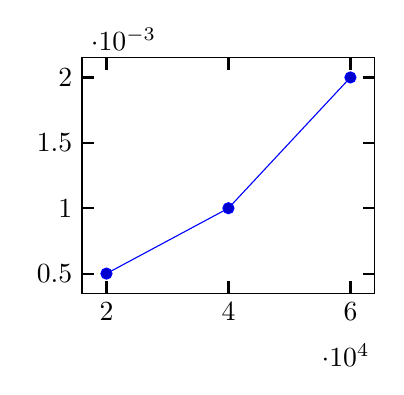
\begin{tikzpicture}
\begin{axis}[scaled ticks=true]
	\addplot coordinates {
		(20000,0.0005)
		(40000,0.0010)
		(60000,0.0020)
	};
\end{axis}
\end{tikzpicture}%
\end{codeexample}

\begin{codeexample}[]
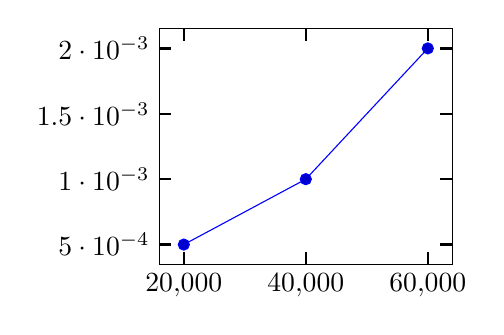
\begin{tikzpicture}
\begin{axis}[scaled ticks=false]
	\addplot coordinates {
		(20000,0.0005)
		(40000,0.0010)
		(60000,0.0020)
	};
\end{axis}
\end{tikzpicture}
\end{codeexample}

	The |scaled ticks| key is a style which simply sets scaled ticks for both, $x$ and $y$.

	The value |base 10:|\meta{e} allows to adjust the algorithm manually. For example, |base 10:3| will divide every tick label by $10^3$:
\begin{codeexample}[]
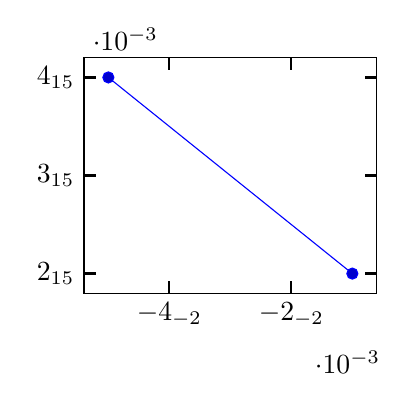
\begin{tikzpicture}
	\begin{axis}[scaled ticks=base 10:3,
		/pgf/number format/sci subscript]
	\addplot coordinates
		{(-0.00001,2e12) (-0.00005,4e12) };
	\end{axis}
\end{tikzpicture}
\end{codeexample}
\noindent Here, the \texttt{sci subscript} option simply saves space.
In general, |base 10:|$e$ will divide every tick by $10^e$. The effect
is not limited by the ``too large or too small'' decisions mentioned
above.

	The value |real:|\meta{num} allows to divide every tick by a fixed \meta{num}.
	For example, the following plot is physically ranged from $0$ to $2\pi$, but the tick scaling algorithm is configured to divide every tick label by $\pi$.
\begin{codeexample}[]
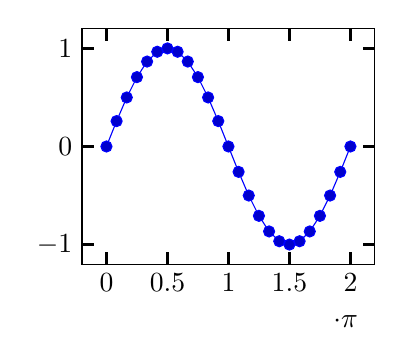
\begin{tikzpicture}
	\begin{axis}[
		xtick={0,1.5708,...,10},
		domain=0:2*pi,
		scaled x ticks={real:3.1415},
		xtick scale label code/.code={$\cdot \pi$}]
	\addplot {sin(deg(x))};
	\end{axis}
\end{tikzpicture}
\end{codeexample}
	\noindent Setting |scaled ticks=real:|\meta{num} also changes the |tick scale label code| to
\begin{codeexample}[code only]
\pgfkeys{/pgfplots/xtick scale label code/.code=
	{$\pgfkeysvalueof{/pgfplots/tick scale binop} \pgfmathprintnumber{#1}$}}.
\end{codeexample}
\noindent The key |tick scale binop| is described below, it is set initially to |\cdot|.

A further -- not very useful -- example is shown below. Every $x$ tick label has been divided by $2$, every $y$ tick label by $3$.
\nobreak
\begin{codeexample}[]
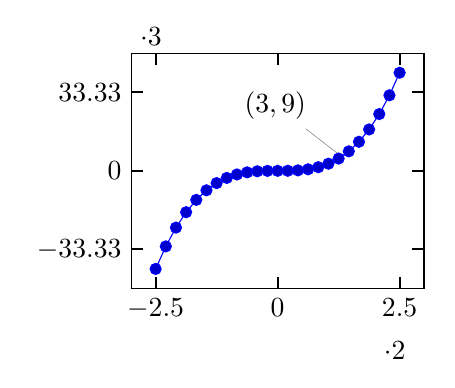
\begin{tikzpicture}
	\begin{axis}[
		scaled x ticks=real:2,
		scaled y ticks=real:3]
	\addplot {x^3};
	\node[pin=135:{$(3,9)$}] at (axis cs:3,9) {};
	\end{axis}
\end{tikzpicture}
\end{codeexample}

	The last option, |scaled ticks=manual:|\marg{label}\marg{code} allows even more customization. It allows \emph{full control} over the displayed scaling label \emph{and} the scaling code: \meta{label} is used as-is inside of the tick scaling label while \meta{code} is supposed to be a one-argument-macro which scales each tick. Example:
\begin{codeexample}[]
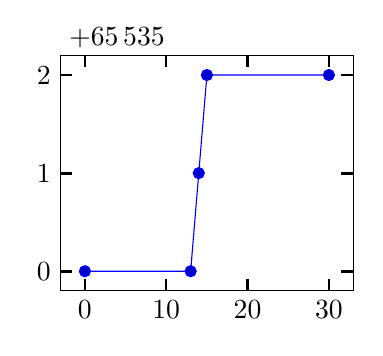
\begin{tikzpicture} 
\begin{axis}[
	% warning: the '%' signs are necessary (?)
	scaled y ticks=manual:{$+65\,535$}{%
		\pgfmathparse{#1-65535}%
	},
	yticklabel style={
		/pgf/number format/fixed,
		/pgf/number format/precision=1},
] 
\addplot coordinates { 
	(0, 65535) 
	(13, 65535) 
	(14, 65536) 
	(15, 65537) 
	(30, 65537) 
}; 
\end{axis} 
\end{tikzpicture} 	
\end{codeexample}
\noindent The example uses |$+65\,535$| as tick scale label content. Furthermore, it defines the customized tick label formula $y - (+6.5535\cdot 10^4) = y - 65535$ to generate $y$ tick labels.

The \meta{label} can be arbitrary. It is completely in user control. The second argument, \meta{code} is supposed to be a one-argument-macro in which |#1| is the current tick position in floating point representation. The macro is expected to assign |\pgfmathresult| (as a number). The \PGF\ manual~\cite{tikz} contains detailed documentation about its math engine.

This feature may also be used do transform coordinates in case they can't be processed with \PGFPlots: transform them and supply a proper tick scaling method such that tick labels represent the original range.

If \meta{label} is empty, the tick scale label won't be drawn (and no space will be occupied).

Tick scaling does \emph{not} work for logarithmic axes.
\end{pgfplotsxykeylist}

\begin{pgfplotsxycodekeylist}{\x tick scale label code}
Allows to change the default code for scaled tick labels. The default is
\begin{codeexample}[code only]
\pgfplotsset{
	xtick scale label code/.code={$\cdot 10^{#1}$}
}
\end{codeexample}

More precisely, it is
\begin{codeexample}[code only]
\pgfplotsset{
	xtick scale label code/.code={$\pgfkeysvalueof{/pgfplots/tick scale binop} 10^{#1}$}
}
\end{codeexample}
\noindent and the initial value of |tick scale binop| is |\cdot|, but it can be changed to |\times| if desired.

If the code is empty, no tick scale label will be drawn (and no space is consumed).
\end{pgfplotsxycodekeylist}

\begin{pgfplotscodekey}{tick scale label code}
	A style which sets |xtick scale label code| and those for $y$ and $z$.
\end{pgfplotscodekey}


\begin{pgfplotskey}{tick scale binop=\marg{\TeX\ math operator} (initially \textbackslash cdot)}
	Sets the binary operator used to display tick scale labels.
\begin{codeexample}[]
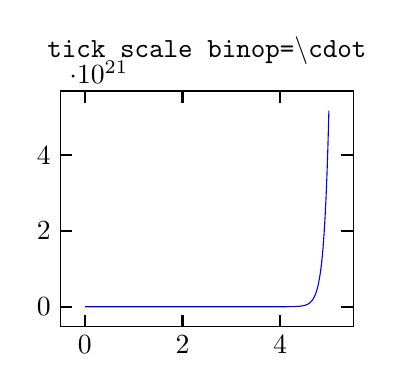
\begin{tikzpicture}
\begin{axis}[
	title=\texttt{tick scale 
		binop=\textbackslash cdot}]
\addplot
	[mark=none,blue,samples=250,
	 domain=0:5]
	{exp(10*x)};
\end{axis}
\end{tikzpicture}
\end{codeexample}

\begin{codeexample}[]
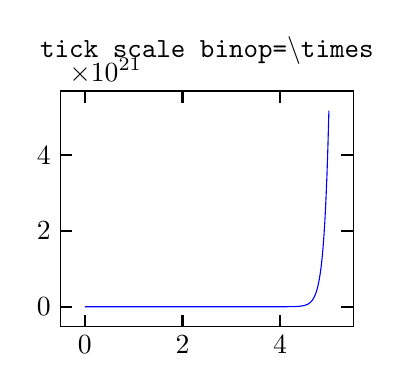
\begin{tikzpicture}
\begin{axis}[
	title=\texttt{tick scale 
		binop=\textbackslash times},
	tick scale binop=\times]
\addplot
	[mark=none,blue,samples=250,
	 domain=0:5] 
	{exp(10*x)};
\end{axis}
\end{tikzpicture}
\end{codeexample}
\end{pgfplotskey}

\makeatletter
\let\itsinitial=\pgfplots@scale@ticks@below@exponent
\makeatother
\begin{pgfplotskey}{scale ticks below exponent=\marg{exponent} (initially \itsinitial)}
Allows fine tuning of the `|scaled ticks|' algorithm: if the axis limits are of magnitude $10^e$ and $e<$\meta{exponent}, the common prefactor~$10^e$ will be factored out. The default is 
\end{pgfplotskey}

\makeatletter
\let\itsinitial=\pgfplots@scale@ticks@above@exponent
\makeatother
\begin{pgfplotskey}{scale ticks above exponent=\marg{exponent} (initially \itsinitial)}
Allows fine tuning of the '|scaled ticks|' algorithm: if the axis limits are of magnitude $10^e$ and $e>$\meta{exponent}, the common prefactor~$10^e$ will be factored out.
\end{pgfplotskey}


\subsubsection{Tick Fine-Tuning}
The tick placement algorithm depends on a number of parameters which can be tuned to get better results.
\begin{pgfplotskey}{max space between ticks=\marg{number} (initially \axisdefaulttickwidth)}
\label{maxspacebetweenticks}
	Configures the maximum space between adjacent ticks in full points. The suffix ``|pt|'' has to be omitted and fractional numbers are not supported.
\end{pgfplotskey}

\begin{pgfplotskey}{try min ticks=\marg{number} (initially \axisdefaulttryminticks)}
	Configures a loose lower bound on the number of ticks. It should be considered as a suggestion, not a tight limit. This number will increase the number of ticks if `|max space between ticks|' produces too few of them.

	The total number of ticks may still vary because not all fractional numbers in the axis' range are valid tick positions.
\end{pgfplotskey}

\begin{pgfplotskey}{try min ticks log=\marg{number} (initially 3)}
	The same as |try min ticks|, but for logarithmic axis.
\end{pgfplotskey}

\begin{pgfplotskeylist}{tickwidth=\marg{dimension} (initially 0.15cm),major tick length=\marg{dimension} (initially 0.15cm)}
	Sets the length of major tick lines. 
	
	It can be accessed using |\pgfkeysvalueof{/pgfplots/major tick length}|.
\end{pgfplotskeylist}

\begin{pgfplotskeylist}{subtickwidth=\marg{dimension} (initially 0.1cm),minor tick length=\marg{dimension} (initially 0.1cm)}
	Sets the length of minor tick lines.

	It can be accessed using |\pgfkeysvalueof{/pgfplots/minor tick length}|.
\end{pgfplotskeylist}

\begin{pgfplotsxykeylist}{\x tick placement tolerance (initially 0.05pt)}
	Tick lines and labels will be placed if they are no more than this tolerance beyond the axis limits. This threshold should be chosen such that it does not produce visible differences while still providing fault tolerance.

	The threshold is given in paper units of the final figure.
\end{pgfplotsxykeylist}

\begin{pgfplotsxykey}{log basis \x=\marg{number} (initially empty)}
	Allows to change the logarithms used for logarithmic axes.

	Changing to a different log basis is nothing but a scale. However, it also changes the way tick labels are displayed: they will also be shown in the new basis.

\begin{codeexample}[]
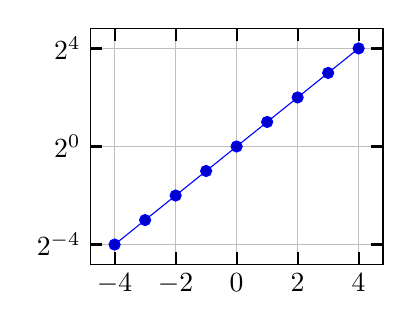
\begin{tikzpicture}
	\begin{semilogyaxis}[log basis y=2,grid=major,samples at={-4,...,4}]
		\addplot {2^x};
	\end{semilogyaxis}
\end{tikzpicture}
~
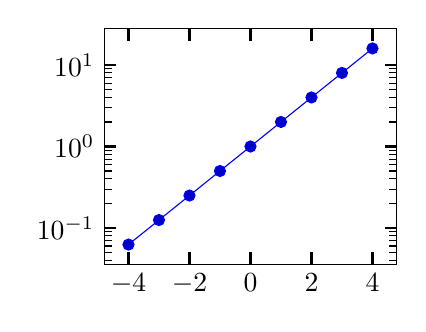
\begin{tikzpicture}
	\begin{semilogyaxis}[log basis y=10,samples at={-4,...,4}]
		\addplot {2^x};
	\end{semilogyaxis}
\end{tikzpicture}
\end{codeexample}
	
	The initial setting is `|log basis x=|' which defaults to: the natural logarithm for any coordinates (basis $\exp(1)$), and the logarithm base $10$ for the display of tick labels.

	If the log basis is changed to something different than the empty string, the chosen logarithm will be applied to any input coordinate (if the axis scale is log as well) and tick labels will be displayed in this basis. 

	In other words: usually, you see log axes base $10$ and that's it. It is only interesting for coordinate filters: 
	the initial setting (with empty \meta{number}) uses coordinate lists basis $e$ although the display will use basis~$10$ (i.e.\ it is rescaled). Any non-empty value \meta{number} causes both, coordinate lists \emph{and} display to use \meta{number} as basis for the logarithm. The javascript code of the |clickable| library will always use the \emph{display} basis (which is usally $10$) when it computes slopes.

	\paragraph{Technical remarks.} When |log basis x| is used, the style |log basis ticks=|\marg{axis char} will be installed (in this case |log basis ticks=x|). This style in turn will change |log number format code|.

	Please note that |xtickten| will be used differently now: it will provide the desired ticks in the new basis! Despite the misleading name ``|ten|'', |xtickten={1,2,3,4}| will yield ticks at $2^1,2^2,2^3,2^4$ if |log basis x=2| has been set.
\end{pgfplotsxykey}
